%%%%%%%%%%%%%%%%%%%%%%%%%%%%%%%%%%%%%%%%%%%%%%%%%%%%%%%%%%%%%%%%%%%%%%%%
\chapter{CONCLUSIONES Y TRABAJO FUTURO}
\label{ch:conclusiones}

\section{Conclusiones}
 El presente trabajo de Fin de Carrera consiste en el desarrollo de una herramienta software para manejar apuestas en Internet bajo los terminales móviles \emph{iOS}. 
 
Uno de los puntos claves del presente trabajo ha sido el portado de un servicio web originalmente diseñado para el mundo de navegadores web de PC a una plataforma móvil de última generación. En este trabajo de fin de carrera se ha elegido el \emph{API} de Betfair y podemos concluir que su portado ha sido exitoso. La clave de este éxito ha sido el diseño e implementación de un \emph{parser}, explicado en el capítulo \ref{ch:implemetacion}, que hace de nexo de unión entre el servidor de Betfair y la aplicación. El \emph{parser} realiza las funciones de un codificador y encapsulador de datos. En torno a él gira el resto del desarrollo.
 
 Se han implementado los servicios básicos del \emph{API}. Está limitación de servicios se ha debido al tipo de licencia elegido. Por este motivo se ha diseñado, desde el primer momento, una aplicación de tipo modular para que en un futuro se agreguen el resto de las funcionalidades sin ningún tipo de complicación. La arquitectura del desarrollo permite este tipo de ampliaciones siguiendo las técnicas de software específicas.
 
 Otro punto clave y diferenciador en este trabajo es la implementación de la funcionalidad de \emph{trading}, como vimos en el capítulo \ref{ch:intro}. La aplicación es capaz de recalcular las condiciones del mercado basándose en una apuesta ya realizada y asistir al usuario para una ganancia segura o minimizar la pérdida según la evolución del mercado. La arquitectura de la aplicación esta diseñada para que en un futuro cercano se pueda desarrollar esta funcionalidad para que se realice sobre múltiples eventos y mercados.
 
 Se ha conseguido no almacenar información localmente redundante de la aplicación. Debido al uso de servicios web todos los datos de consulta y de generación por parte del usuario se guardan en el servidor. Por lo tanto, si el usuario usa alguna otra aplicación en otra plataforma no sería necesario ningún mecanismo de sincronización de información. En este tipo de contextos es mejor disponer de datos lo más actualizados posibles directamente desde el servidor que manejar una caché de datos desactualizadas al poco tiempo de descargarse del servidor. Los mercados están en continua evolución.
 
 Otro objetivo cumplido es la implementación de la internacionalización de la aplicación. La aplicación estará disponible a través de la tienda \emph{iTunes} \emph{Store}. Esta tienda tiene un acceso mundial y debido a ello se ha adoptado los principales idiomas para que la aplicación sea lo más extendida posible. 
 
\section{Trabajo futuro}
 Como ya hemos visto en la arquitectura de la aplicación, el sistema está preparado para posibles futuras funcionalidades extras que podemos aportar con los datos que nos ofrece el \emph{API}. Debido a que el núcleo de la aplicación es la obtención y proceso de la información contenida en Betfair, cualquier desarrollador puede añadir una funcionalidad extra usando los datos anteriores y acoplarlas fácilmente a la arquitectura de la aplicación. Al usar el modelo vista-controlador, la sencillez a la hora de implementar nuevas funcionalidades está mas que probada.
 
\subsection*{\emph{Trading} global por lista de eventos}
 Una mejora interesante a implementar en un futuro sería la de poder realizar \emph{trading} sobre un mercado entero. Al principio del presente trabajo hemos definido el \emph{trading} como apostar a favor y en contra de un evento determinado para, según nuestra primera apuesta, obtener beneficio seguro o minimizar la pérdida. Pero, apostar a favor de un evento ¿puede suponer que éste afecte al resto del mercado? Pongamos un ejemplo, supongamos que estamos apostando por quién va a ser el campeón del mundial de fútbol de Sudáfrica. Apostar a favor de un equipo puede llevar la consecuencia de apostar en contra de los restantes participantes si en vez de pensar en un equipo concreto pensamos en el mercado completo. 
 
  Este cambio en nuestro planteamiento supone llevar a cabo un gran control sobre todas las variables que afectan al mercado completo y no sólo por un evento. Para poder analizar completamente los datos de mercado (cuota y precio) necesitamos analizar los datos concretos de cada evento de dicho mercado. Para poder obtener cual sería el conjunto de apuestas a realizar en el mercado para obtener el beneficio tenemos que resolver un conjunto de ecuaciones lineales que representan al mercado cuyas incógnitas serán las cuotas y cantidad a apostar por cada eventos de dicho mercado.    
  
 Normalmente los mercados tienen unos 30 eventos. Para poder obtener una solución óptima tenemos que echar mano de herramientas de software de resolución de ecuaciones lineales, tales como \lstinline{zympl} y \lstinline{glpsol}. 
  
  
  
   La idea es tener una máquina servidora capaz de realizar estos cálculos cada, pongamos por ejemplo, una hora. Se trata de analizar continuamente el mercado para encontrar el momento idóneo para el \emph{trading} global. El incluir otra máquina a parte del terminal es debido a la restricción de la batería. Si hiciéramos uso del terminal para estos cálculos reduciría drásticamente la vida útil de la misma. La máquina avisaría a la aplicación móvil del terminal en cuanto encontrase una solución adecuada a los parámetros configurados. 
   
    El procedimiento por el cual el usuario es notificado con la solución es implementar la solución de mensajería tipo \emph{push} de Apple en el \emph{iPhone}. A continuación mostramos como son las notificaciones en el terminal, también como mejora a añadir al proyecto.
    
 \subsubsection*{Notificación por mensajes \emph{Push} de Apple}
   
   En un modelo típico de cliente-servidor, el cliente es el encargado de contactar con el servidor para la descarga de nuevos datos, como por ejemplo el servicio de correo electrónico. En un dispositivo móvil, el cuál siempre tiene el inconveniente de la batería, esta solución no es válida debido al consumo energético en cada consulta al servidor. Para estos casos las notificaciones \emph{push} son las solución a este dilema. Una notificación \emph{push} es un mensaje corto que el servidor envía al cliente para notificarle que tiene datos para ser descargados o eventos pendientes tales como nueva versión de la aplicación. 
   
    Cuando un dispositivo móvil recibe una notificación de una aplicación que no está ejecutada en ese momento, el sistema notifica al usuario a través de un mensaje de alerta, un sonido determinado o un número indicador en el icono de la aplicación (o una combinación de este conjunto) de un evento a tratar por parte del usuario. El usuario, en todo momento, tiene la posibilidad de ejecutar la aplicación para obtener los datos notificados o simplemente ignorar el mensaje.

     \begin{figure}[h!]
    \centering
       
\includegraphics[width=0.2\textwidth]{./images/badged_app.jpg}
     \caption{Alerta tipo 1 }
   \label{fig:Alerta 1}
\end{figure}

\begin{figure}[h!]
    \centering
       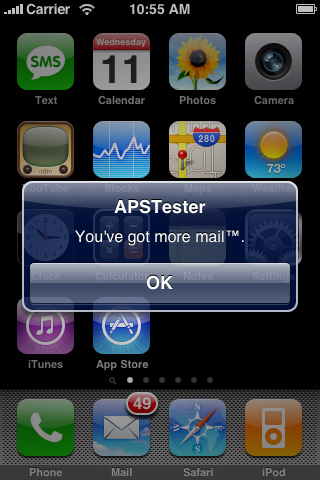
\includegraphics[width=0.3\textwidth]{./images/notif_msg_one_button.jpg}
     \caption{Alerta tipo 2 }
   \label{fig:Alerta 2}
\end{figure}

\begin{figure}[h!]
    \centering
       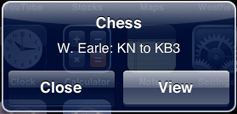
\includegraphics[width=0.3\textwidth]{./images/alert.jpg}
     \caption{Alerta tipo 3 }
   \label{fig:Alerta 3}
\end{figure}

     
    Brevemente explicaremos el proceso completo del envío de un mensaje desde el servidor hasta la aplicación cliente del terminal. 
    
    En todo el proceso intervienen 3 actores: el servidor que desea entregar un mensaje, el servidor de Apple de envío de mensajes y la aplicación cliente.
    
 \begin{figure}[h!]
    \centering
       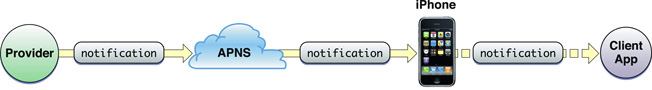
\includegraphics[width=0.95\linewidth]{./images/remote_notif_simple.jpg}
     \caption{Proceso general }
   \label{fig:Notificacion proceso}
\end{figure}

   \subsubsection*{Registro}

     El primer paso del proceso es el registro de la aplicación en el servidor de Apple para activar el servicio de notificaciones. Tal y como se muestra en la figura \ref{fig:Notificacion Registro}, la aplicación cliente se conecta al \emph{APNS}\footnote{Apple Push Notification Server, el servidor encargado de recibir y enviar el mensaje de un tercero a un terminal \emph{iPhone}} para la obtención de un identificador (\emph{token}) único para cada aplicación cliente y terminal. El \emph{APNS}, después de comprobar las credenciales del terminal, genera y registra el \emph{token} a partir del \emph{ID} del dispositivo y devuelve al terminal su \emph{token} generado. Este \emph{token} identifica al terminal y por lo tanto lo ha de usar nuestro servidor para poder enviar a este terminal un mensaje \emph{push}. Por eso, el último paso del registro es notificar al servidor desde el terminal el \emph{token} generado para su registro interno.
     
 \begin{figure}[h!]
    \centering
       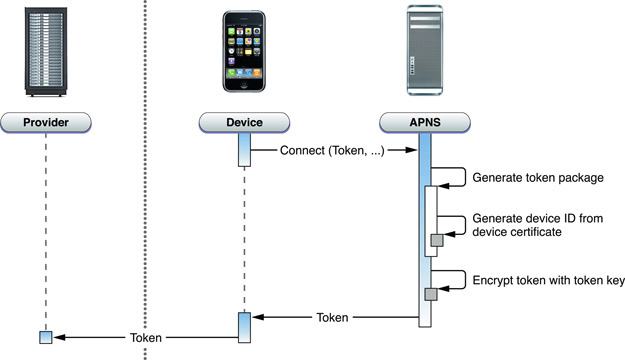
\includegraphics[width=0.8\textwidth]{./images/token_generation.jpg}
     \caption{Registro }
   \label{fig:Notificacion Registro}
\end{figure}
  
     \subsubsection*{Envío de una notificación}
     
     Tal y como se muestra en la figura \ref{fig:Notificacion envio} cuando el servidor requiere enviar una notificación a un cliente determinado para indicarle que dispone de datos nuevos que descargar, éste envía el mensaje en cuestión junto con el identificador del terminal al \emph{APNS}. El servidor \emph{APNS} comprueba que el \emph{token} ha sido generado por un certificado válido y que identifica a un terminal registrado previamente. Si todo esta correcto le envía el mensaje a la aplicación cliente del terminal.
     
 \begin{figure}[h!]
    \centering
       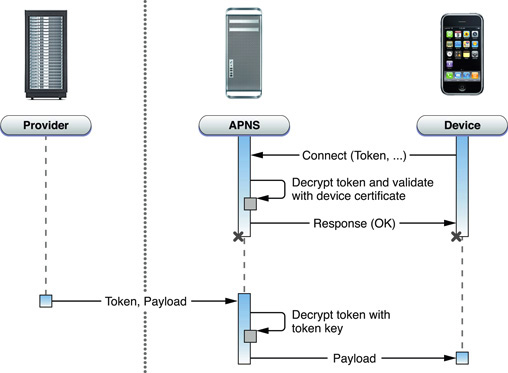
\includegraphics[width=0.8\textwidth]{./images/token_trust.jpg}
     \caption{Envío}
   \label{fig:Notificacion envio}
\end{figure}

 Como podemos ver, mediante estas notificaciones podemos tener al cliente lo más actualizado posible minimizando el gasto de batería si le tuviese que conectar periódicamente con algún servidor. \cite{betfair:web}

%%% Local Variables: 
%%% mode: latex
%%% TeX-master: "tfc-betfair-ios"
%%% TeX-PDF-mode: t
%%% ispell-local-dictionary: "castellano"
%%% End: 
